% \newtheorem{claim}[theorem]{Claim}
\newtheorem{proposition}[theorem]{Proposition}
% \newtheorem{corollary}[theorem]{Corollary}
\newtheorem{conjecture}[theorem]{Conjecture}
\newtheorem{goal}[theorem]{Goal}

% \theoremstyle{definition}
% \newtheorem{example}[theorem]{Example}
% \newtheorem*{fact}{Fact}

% \theoremstyle{definition}
% \newtheorem{question}[theorem]{Question}
% \newtheorem*{unquestion}{Question}

% \theoremstyle{remark}
% \newtheorem*{remark}{Remark}
% \newtheorem*{proofsketch}{Outline of proof}

% \theoremstyle{definition}
% \newtheorem{definition}[theorem]{Definition}

\newcommand{\pmf}{\mathbb{P}\mathcal{MF}}
\newcommand{\mf}{\mathcal{MF}}
\newcommand{\mcg}{\text{MCG}}
\newcommand{\os}{\mathcal{S}}
\newcommand{\no}{\mathcal{N}}
\newcommand{\teich}{\mathcal{T}}
\newcommand{\mg}{\mathcal{M}}
\newcommand{\pslr}{\text{PSL}(2, \mathbb{R})}
\newcommand{\scc}{\mathscr{S}}
\newcommand{\QQ}{\mathbb{Q}}
\newcommand{\ZZ}{\mathbb{Z}}
\newcommand{\wt}{\widetilde}
\newcommand{\cA}{\mathcal{A}}
\newcommand{\cR}{\mathcal{R}}
\newcommand{\dynlim}{\Lambda_{\text{dyn}}}
\newcommand{\geolim}{\Lambda_{\text{geo}}}
\newcommand{\HH}{\mathbb{H}^2}
\newcommand{\RR}{\mathbb{R}}
\newcommand{\expansion}{\text{Sat}}
\newcommand{\err}[1]{\text{err}_{#1}}
\newcommand{\norm}[1]{\left\lVert#1\right\rVert}
\newcommand{\dd}{\text{\,d}}
\newcommand{\lhyp}{\ell_{\text{hyp}}}
\newcommand{\lflat}{\ell_{\text{flat}}}
\renewcommand{\qedsymbol}{}


\newcommand\Narrower[2][3em]{%
\makebox[\linewidth][c]{%
  \begin{minipage}{\dimexpr\textwidth-#1\relax}
  \raggedright#2
  \end{minipage}%
  }%
}

\def\signed #1{{\leavevmode\unskip\nobreak\hfil\penalty50\hskip2em
  \hbox{}\nobreak\hfil(#1)%
  \parfillskip=0pt \finalhyphendemerits=0 \endgraf}}

\newsavebox\mybox
\newenvironment{aquote}[1]
  {\savebox\mybox{#1}\begin{quote}}
  {\signed{\usebox\mybox}\end{quote}}


\setbeamercolor{block title}{fg=black, bg=pink}

\title{Dynamics on the Moduli Space of Non-Orientable Surfaces}
\author[Sayantan Khan]{Sayantan Khan}
\institute{University of Michigan}

% \newdate{date}{2}{4}{2024}
\date{Tuesday, April 2\textsuperscript{nd} 2024}

\subject{Mathematics}

% \setbeamertemplate{footline}[page number]{}

% Delete this, if you do not want the table of contents to pop up at
% the beginning of each subsection:
% \AtBeginSection[]
% {
%   \begin{frame}<beamer>{Outline}
%     \tableofcontents[currentsection]
%   \end{frame}
% }


\begin{document}

\begin{frame}
  \titlepage
\end{frame}

\section{Moduli spaces of non-orientable surfaces}

\begin{frame}
\begin{columns}
\begin{column}{0.5\textwidth}
  \begin{center}
    Orientable surfaces \\
    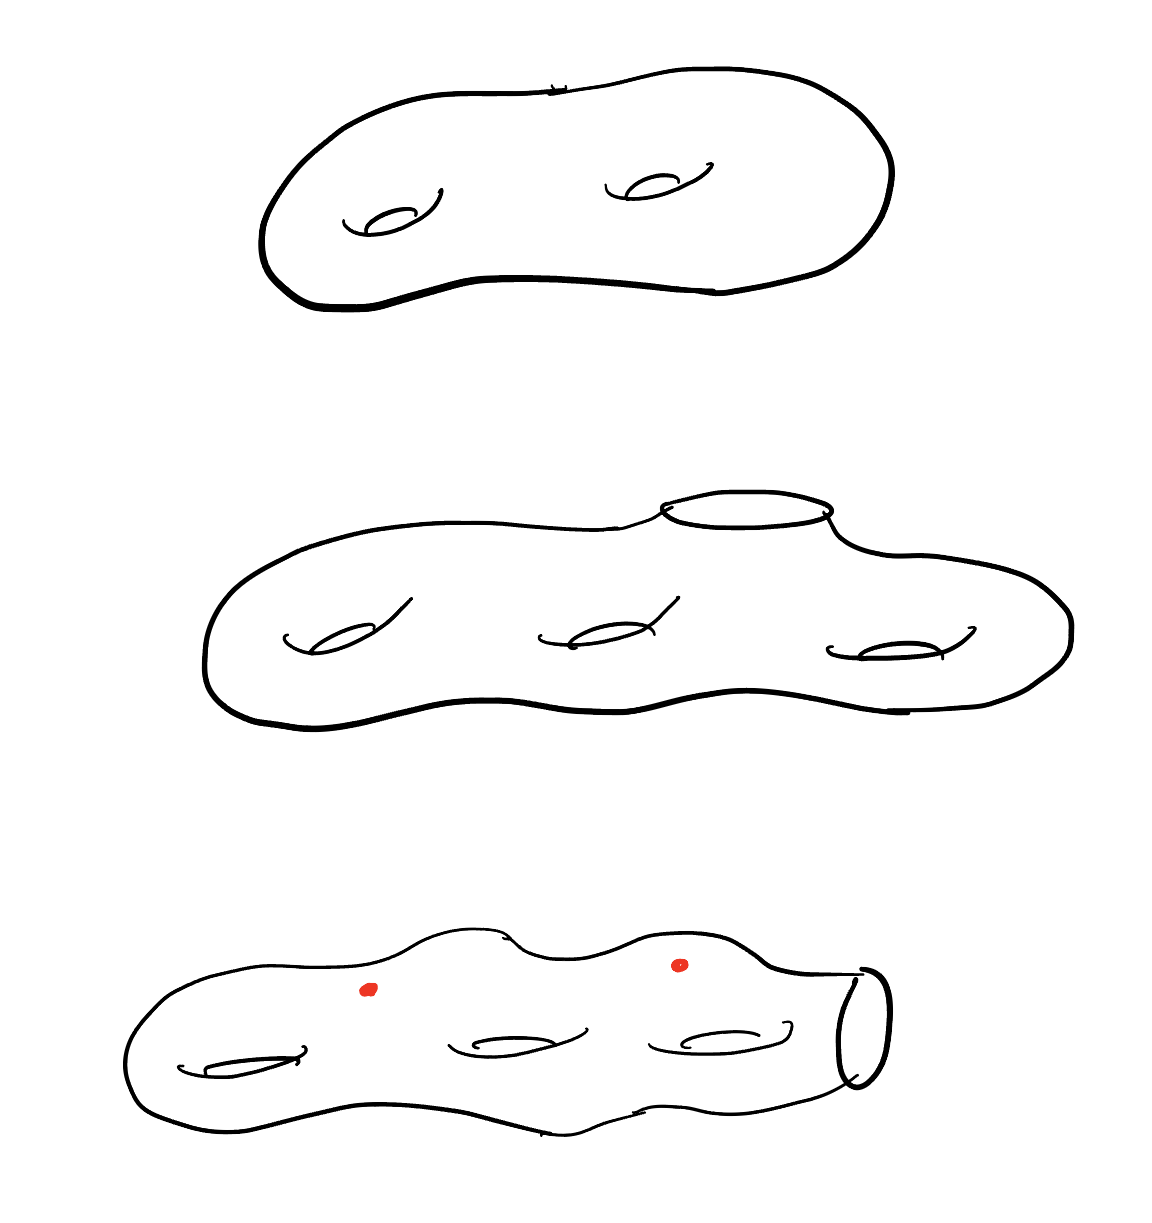
\includegraphics[scale=0.15]{orientable.png}
  \end{center}
\end{column}
\pause
\begin{column}{0.5\textwidth}  %%<--- here
    \begin{center}
      Non-orientable surfaces
      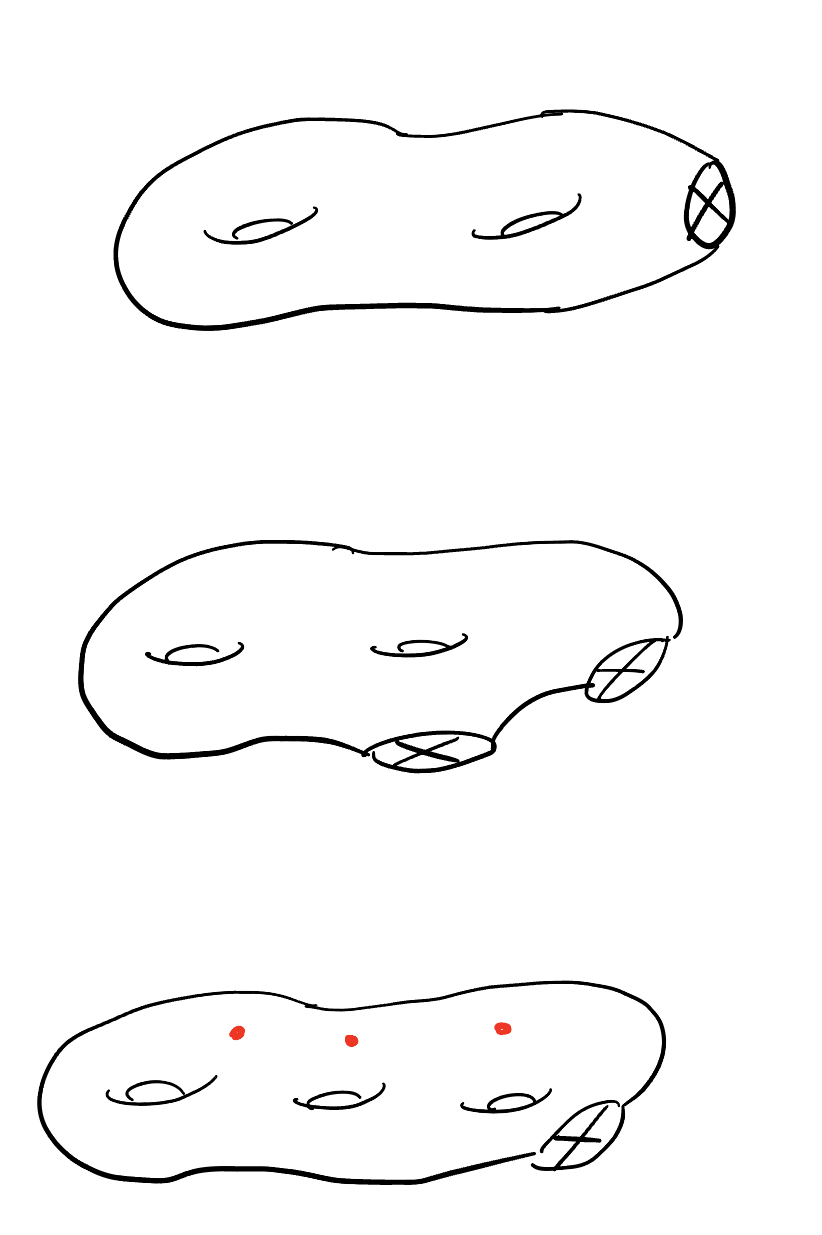
\includegraphics[scale=0.15]{nonorientable.png}
     \end{center}
\end{column}
\end{columns}
\end{frame}

\begin{frame}
  \begin{goal}
    Understand the collection of geometric structures we can put on a topological surface.
  \end{goal}
  \pause
  In particular, understand the set of metrics on a surface with curvature $-1$.
  \begin{figure}[h]
    \centering
    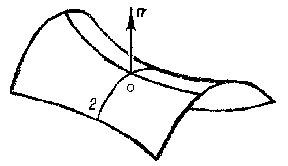
\includegraphics[scale=0.5]{negative-curvature.png}
  \end{figure}
\end{frame}

\begin{frame}
  \begin{align*}
    \mg(\os_g) = \left\{ \text{Curvature $-1$ metrics on $\os_g$} \right\}
  \end{align*}
  \begin{itemize}
  \item<2-> $\mg(\os_g)$ is $6g-6$ dimensional.
  \item<3-> $\mg(\os_g)$ is a metric space: $x$ and $y$ in $\mg(\no_g)$ are close if the derivative of some map $x \to y$ maps circles to ``almost'' circles.
  \item<4-> Unit (co)tangent bundle of $\mg(\os_g)$ is non-compact, but finite volume, and admits a geodesic flow (and an $SL(2, \mathbb{R})$ action) with good dynamical properties.
  \end{itemize}
  \uncover<5->{
  \textbf{Guiding principle}: Dynamics on (co)tangent bundle should have analogies with dynamics of the $SL(2, \mathbb{R})$ action on $SL(2, \mathbb{R})/SL(2, \mathbb{Z})$.
  }
\end{frame}

\begin{frame}
  \begin{align*}
    S^1 \mg(\os_g) = \left\{ \text{Area $1$ half-translation surface structures on $\os_g$} \right\}
  \end{align*}
  \uncover<2->{
    \begin{figure}[h]
      \centering
      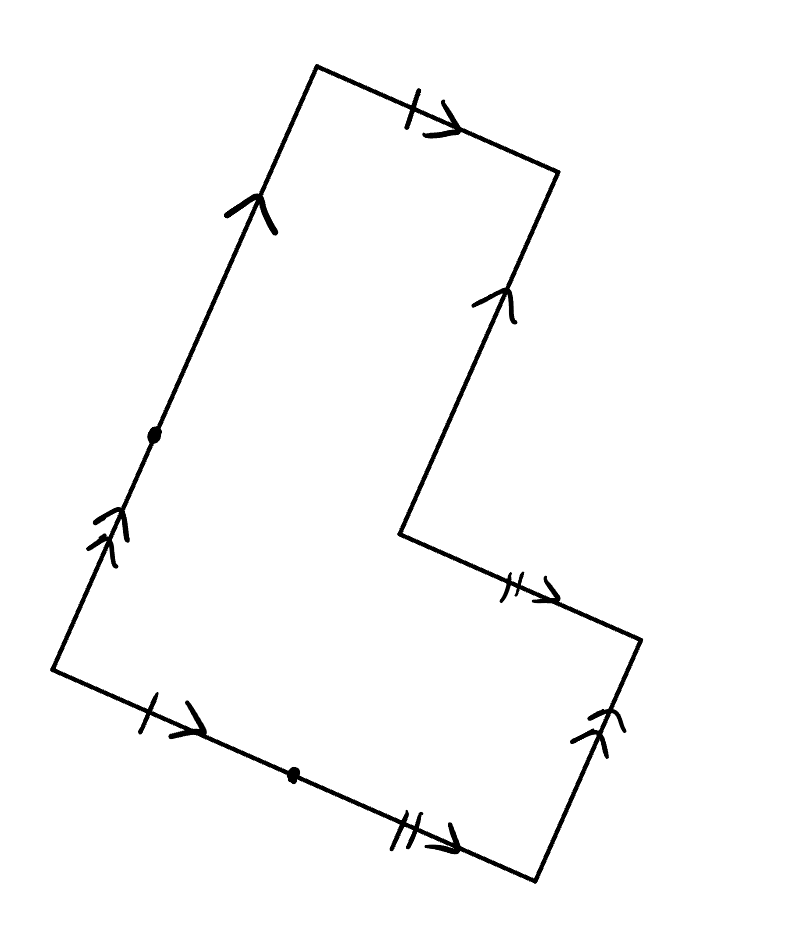
\includegraphics[scale=0.1]{tangent.png}
    \end{figure}
  }

  \uncover<3->{
    \begin{theorem}[Masur's criterion]
      If the vertical flow on translation surface is not uniquely ergodic, then the geodesic ray in $\mg(\os_g)$ escapes to infinity.
    \end{theorem}
  }
\end{frame}

\begin{frame}
  \begin{align*}
    \mg(\no_g) = \left\{ \text{Curvature $-1$ metrics on $\no_g$} \right\}
  \end{align*}
  \begin{itemize}
  \item<2-> $\mg(\no_g)$ is $3g-6$ dimensional.
  \item<3-> $\mg(\no_g)$ is a metric space, with a similarly defined metric.
  \item<4-> Unit (co)tangent bundle of $\mg(\no_g)$ is non-compact, and also infinite volume (with respect to the canonical volume form).
  \item<5->  $S^1 \mg(\no_g)$ admits a geodesic flow but not an $SL(2, \mathbb{R})$ action: however, the dynamical properties are not great.
  \end{itemize}
  \uncover<6->{
  \textbf{Guiding principle?}
  }
\end{frame}

\begin{frame}
  \begin{goal}
    Analyze generic tangent vector in $S^1 \mg(\no_g)$.
  \end{goal}
  \begin{itemize}
  \item<2-> Analyze vertical flow on translation surface.
  \item<3-> Will suffice to look at first return map to a horizontal arc.
  \end{itemize}
    \begin{figure}[h]
      \begin{overprint}
      \centering
      \onslide<4|handout:1>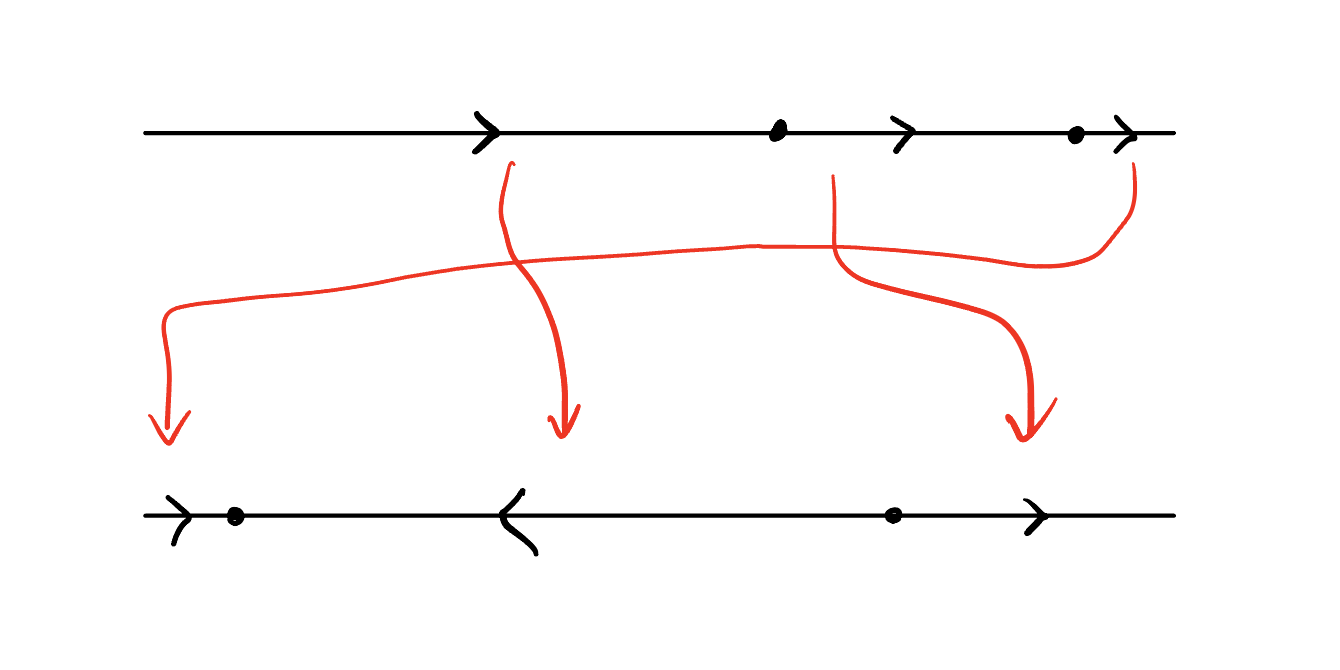
\includegraphics[scale=0.2]{ietwf.png}
      \onslide<5-|handout:2>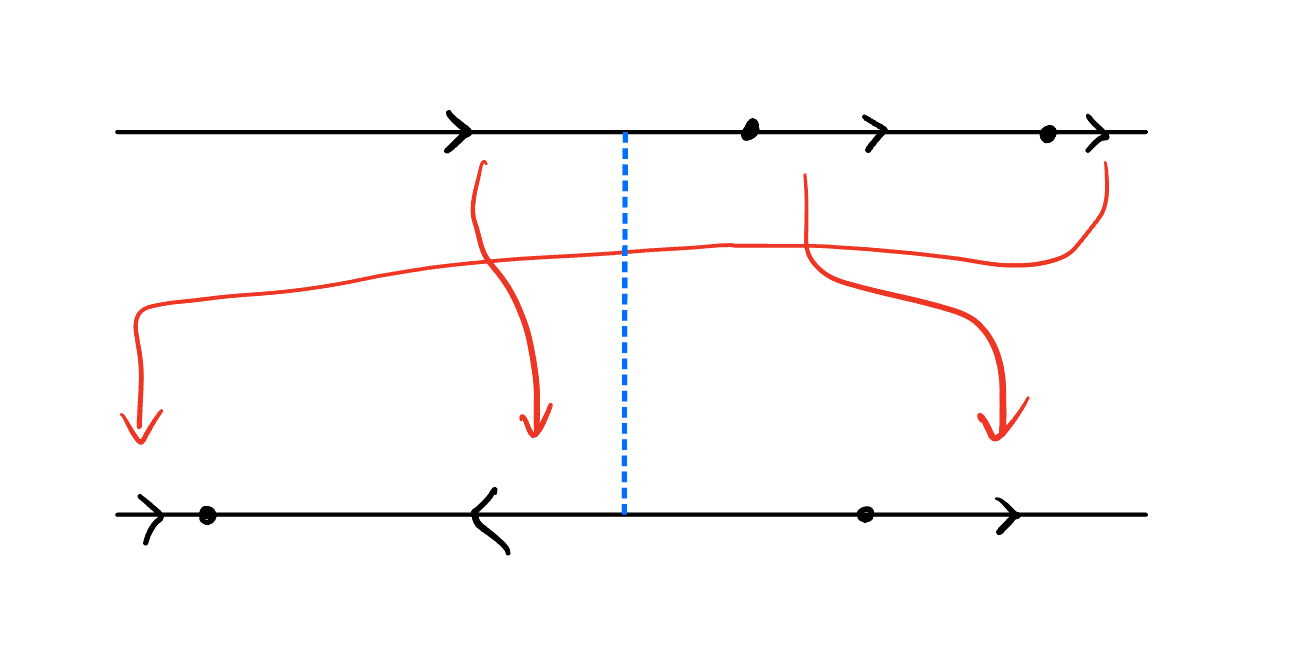
\includegraphics[scale=0.2]{ietwf2.png}
      \end{overprint}
    \end{figure}
    \uncover<6->{
      \begin{theorem}
        Almost every geodesic in $S^1\mg(\no_g)$ escapes to infinity.
      \end{theorem}
    }

\end{frame}

\begin{frame}
 \begin{columns}
\begin{column}{0.5\textwidth}
  \begin{center}
    $\mcg(\no_g)$-action on $\teich(\no_g)$ \\
  \end{center}
  \begin{itemize}
  \item<2-> $\mcg(\no_g)$ is finitely generated.
  \item<3-> The action is infinite covolume.
  \item<4-> Almost no geodesics recur.
  \item<10-> \textbf{Question}: What is the limit set for the $\mcg(\no_g)$ action?
  \item<12-> \textbf{Question}: Can we construct a Patterson-Sullivan measure on the limit set with ``good'' dynamical properties?
  \end{itemize}
\end{column}
\uncover<5-> {
\begin{column}{0.5\textwidth}  %%<--- here
    \begin{center}
      Geometrically finite $\Gamma$ action on $\mathbb{H}$
     \end{center}
     \begin{itemize}
     \item<6-> $\Gamma$ is finitely generated.
     \item<7-> $\Gamma$ action is infinite covolume (with respect to the Liouville measure).
     \item<8-> Almost no geodesics recur.
     \item<9-> Limit set of $\Gamma$ is a subset of the boundary with smaller Hausdorff dimension.
     \item<11-> Have a Patterson-Sullivan measure on the limit set with ``good'' dynamical properties.
     \end{itemize}
\end{column}
}

\end{columns}
\uncover<13->{
  \begin{theorem}[K., Erlandsson-Gendulphe-Pasquinelli-Souto]
    The limit set of the $\mcg(\no_g)$ action on $\teich(\no_g)$ is $\pmf^+(\no_g)$.
  \end{theorem}
}
\end{frame}

\section{Statistical convex-cocompactness}

\begin{frame}
  \frametitle{What do we need for ``good'' Patterson-Sullivan measures?}
  \begin{itemize}
  \item<2-> Classically, Patterson-Sullivan measures were constructed for hyperbolic spaces.
  \item<3-> Then variable negative curvature, Gromov hyperbolic, $\mathrm{CAT}(k)$ for $k \leq 0$, etc.
  \item<4-> Teichmüller spaces are not hyperbolic on the nose, but somewhat hyperbolic.
  \end{itemize}
 \begin{columns}
   \uncover<5-> {
\begin{column}{0.5\textwidth}
  \begin{center}
     \textbf{Thick part}
  \end{center}
  \begin{itemize}
  \item<6-> Region where all curves on underlying surface are longer than $\varepsilon$.
  \item<7-> Geometry of thick region mostly governed by curve complex of surface, which is hyperbolic.
  \end{itemize}
  \vspace{4.4cm}
\end{column}
   }

\uncover<8-> {
\begin{column}{0.5\textwidth}  %%<--- here
    \begin{center}
      \textbf{Thin part}
     \end{center}
     \begin{itemize}
     \item<9-> Region where some curve $\gamma$ on underlying surface is shorter than $\varepsilon$.
     \item<10-> Metric in this region is $L^{\infty}$ product of metrics on subsurfaces (Minsky's product region theorem).
     \end{itemize}
     \uncover<11->{
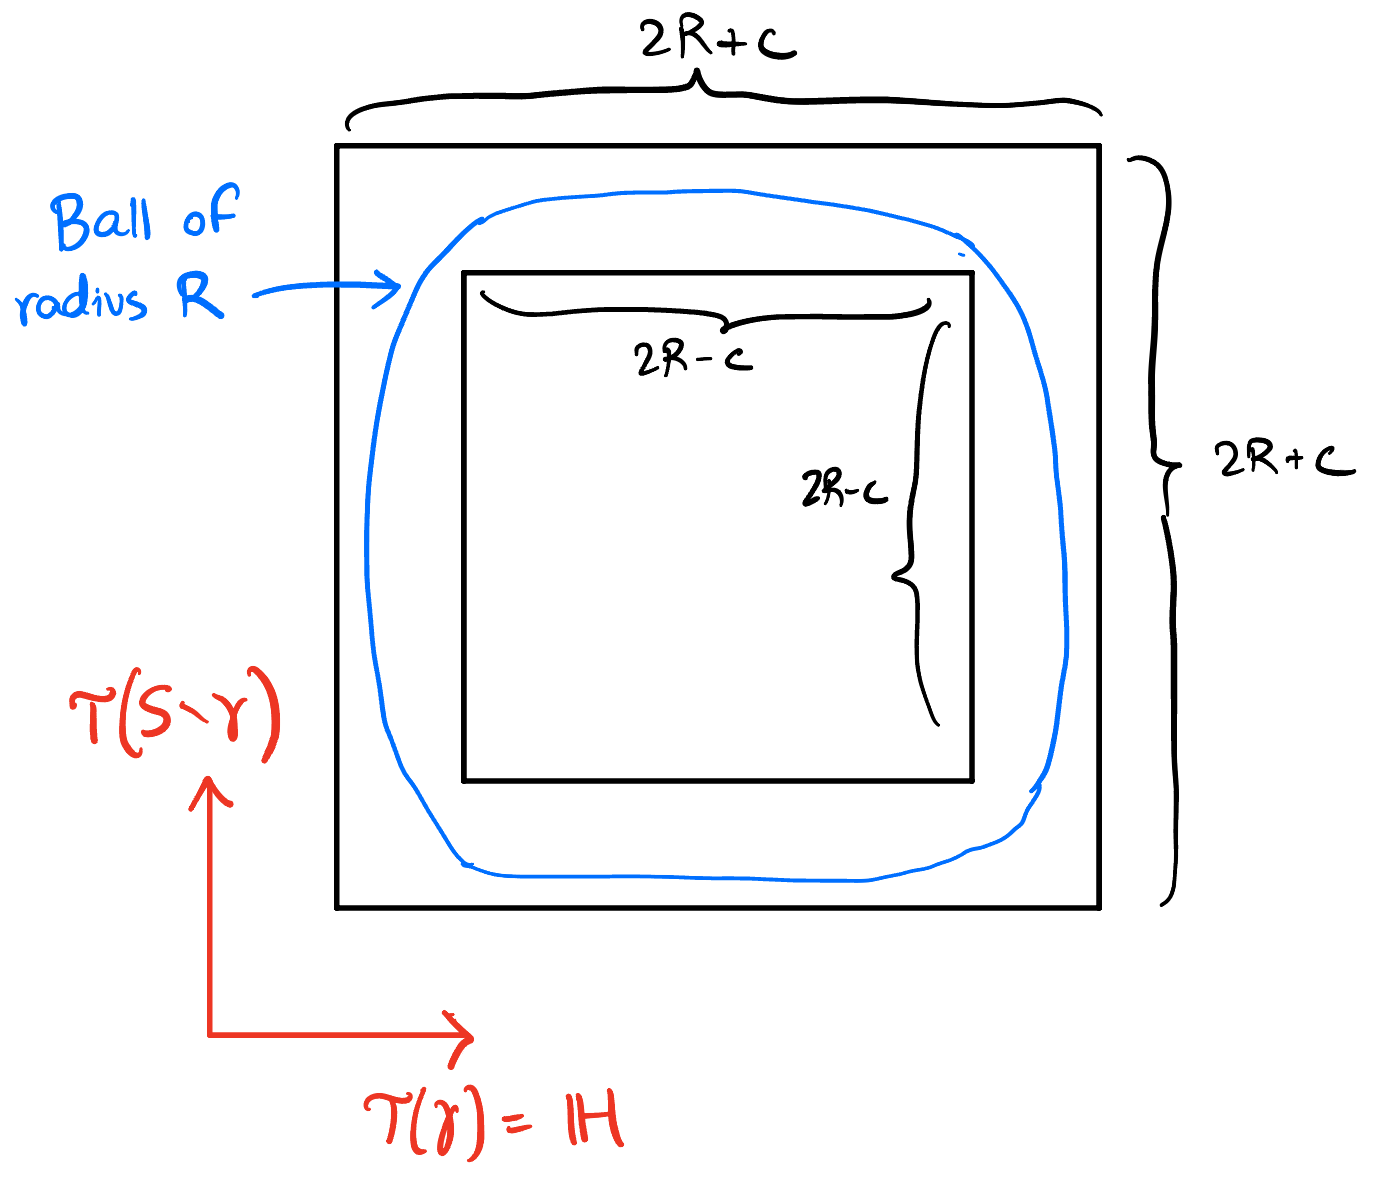
\includegraphics[scale=0.1]{minsky.png}
     }
\end{column}
}

\end{columns}
\end{frame}

\begin{frame}
  \frametitle{Statistical convex-cocompactness}
  \begin{itemize}
  \item<2-> Suffices to show geodesics enter the thin part with exponentially low probabilities. This is the notion of \emph{statistical convex-cocompactness}, and Coulon and Yang showed that this is enough for ``good'' Patterson-Sullivan theory.
  \item<3-> For Teichmüller spaces of orientable surfaces, Eskin and Mirzakhani proved statistical convex-cocompactness.
  \item<4-> They did this by studying a random walk on Teichmüller space instead, and show good recurrence properties for the random walk.
  \item<5-> There are two obstructions in adapting their random walk based techniques to the non-orientable setting.
  \item<6-> Obstruction $1$: Thin region where some \emph{one-sided curve} gets short does not have good recurrence properties for the random walk.
    \uncover<7-> {
      \begin{theorem}[K.]
        The map $(\mathcal{T}_{\varepsilon_t}^{-}(\no_g), \text{induced path metric}) \to (\mathcal{T}_{\varepsilon_t}^{-}(\no_g), \text{Teichmüller metric})$ is $(1 + \varepsilon_d)$ bi-Lipschitz.
      \end{theorem}
    }
  \item<8-> Obstruction 2: It's not obvious that the volume growth entropy of $\mathcal{T}_{\varepsilon_t}^{-}(\no_g)$ is equal to the lattice point growth entropy for the $\mcg(\no_g)$ action.
  \end{itemize}
\end{frame}

\begin{frame}
  \frametitle{How to understand random walks on Teichmüller space}
  \begin{itemize}
  \item<2-> Random walk is with respect to a net in $\teich(\no_g)$: the Teichmüller metric controls the law of the random walk.
  \item<3-> In the thin part, we understand the Teichmüller metric really well, thanks to Minsky.
    \uncover<4-> {
      \begin{figure}[h]
        \centering
        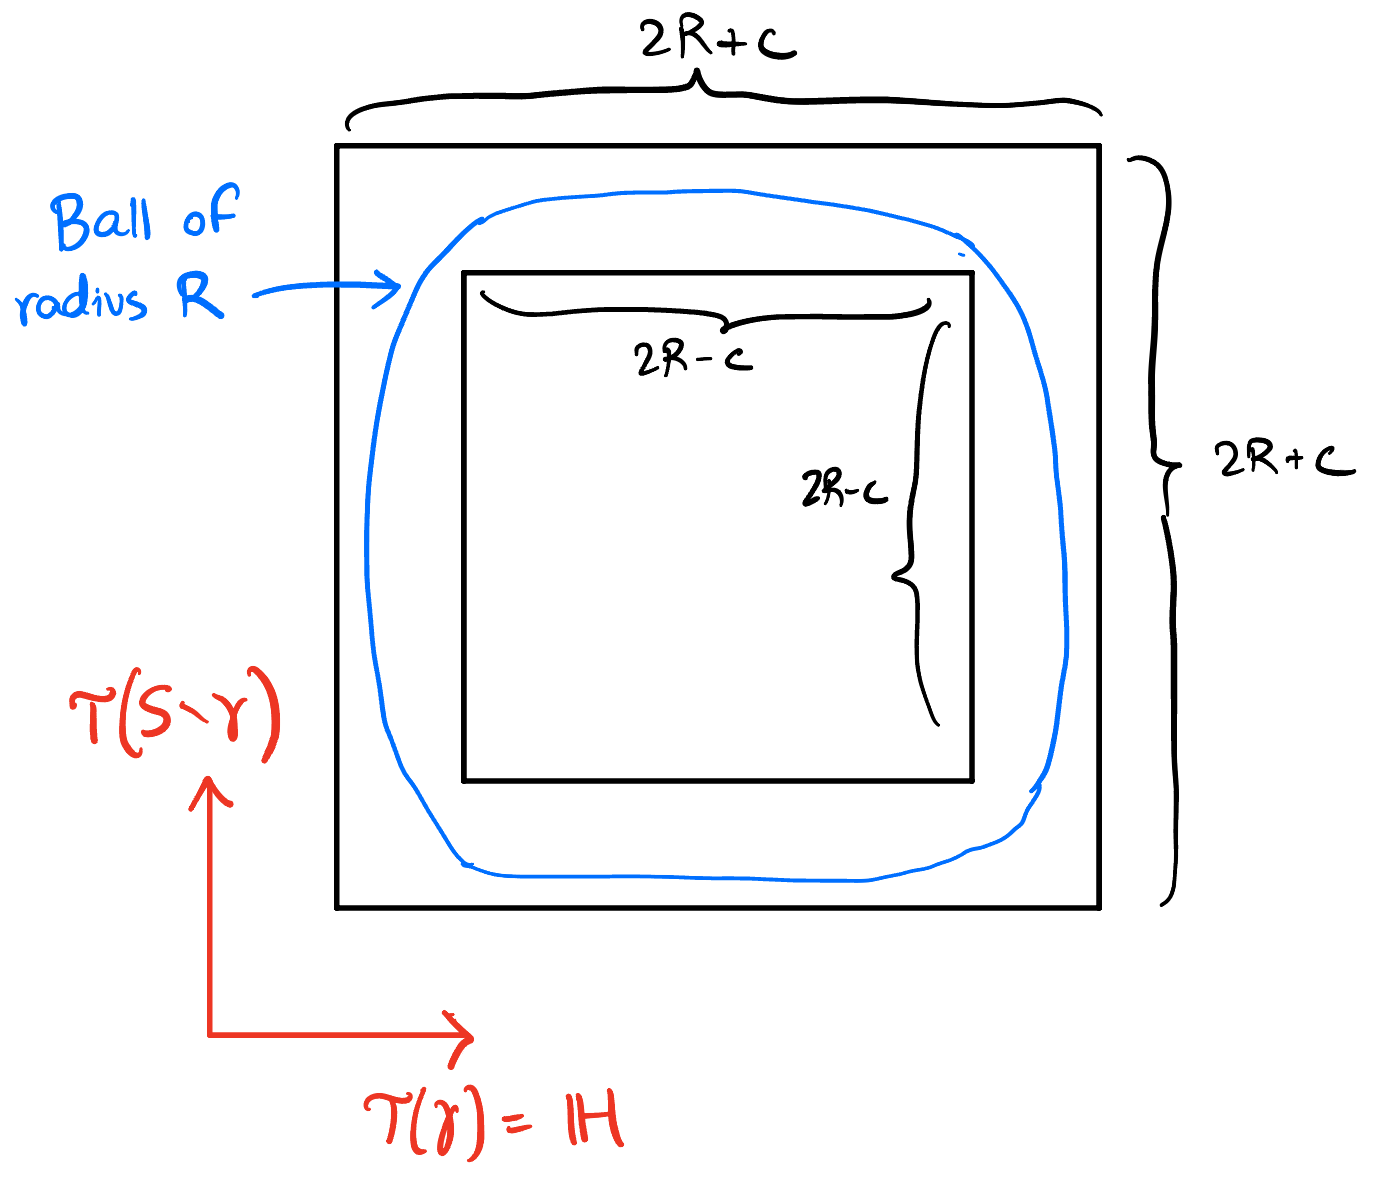
\includegraphics[scale=0.1]{minsky.png}
      \end{figure}
    }
  \item<5-> Since the ball is approximately an $L^{\infty}$ product, picking a point uniformly at random is equivalent to picking a points \emph{independently} on the two coordinates.
  \item<6-> We can show strong recurrence for random walks on a horoball in $\mathbb{H}$.
  \item<7-> For one-sided thin regions, we get a symmetric random walk on $\mathbb{Z}$, which is not strongly recurrent.
  \end{itemize}
\end{frame}

\begin{frame}
  \frametitle{Volume entropy vs lattice point entropy}
  \begin{itemize}
  \item<2-> The random walk argument gives us an estimate in terms of the volume growth entropy. Statistical convex cocompactness requires an estimate in terms of lattice point entropy.
  \item<3-> Hope: the entropies might be equal since $\teich_{\varepsilon_t}^{-}(\no_g)/\mcg(\no_g)$ has finite volume.
  \item<4-> Technical tool to prove a statement like this was invented recently by Dowdall and Masur: \emph{complexity length}.
  \item<5-> Key idea is based off of Minsky's theorem again: we need to understand how volume grows in product region, and therefore, a horoball.
    \uncover<6-> {
      \begin{align*}
        \text{Volume growth for ball of radius $R$ in $\mathbb{H}$} \sim \exp(2R)
      \end{align*}
    }
    \uncover<7-> {
      \begin{align*}
        \text{Volume growth for ball of radius $R$ intersected with a horoball}  \sim \exp(R)
      \end{align*}
    }
  \item<8-> Gap in exponential growth rates tells us that the thin part does not contribute a significant fraction of total volume.
    \uncover<9->{
      \begin{theorem}[K.]
        For all surfaces $S$, and any $\varepsilon_t > 0$, we have the following equality of entropies.
        \begin{align*}
          h_{V}(\teich_{\varepsilon_t}^-(S)) = h_{LP}(\teich_{\varepsilon_t}^-(S))
        \end{align*}
      \end{theorem}
    }
    \uncover<10->{
      \begin{theorem}[K.]
        The action of $\mcg(\no_g)$ on $\teich_{\varepsilon_t}^-(\no_g)$ is statistically convex-cocompact.
      \end{theorem}
    }
  \end{itemize}
\end{frame}

\end{document}

%%% Local Variables:
%%% TeX-master: "presentation"
%%% End: